% ================================================================== 3
\section{Modelo Relacional}

\subsection{Modelo Relacional}

El esquema tiene 18 relaciones: 15 provienen de las entidades del modelo conceptual, dos implementan relaciones con atributos propios (\tb{Aplicacion\_Insumo} y \tb{Mantenimiento}) y una es la bitácora técnica \tb{Auditoria\_Campania}. Las claves primarias van subrayadas y las claves foráneas en cursiva, con una flecha hacia la tabla referenciada. La lista se generó desde el catálogo de PostgreSQL, por lo que coincide exactamente con lo implementado.

%%ESQUEMA_RELACIONAL%%

\subsection{Especificaciones de transformación}

\subsubsection{Entidades}

Cada entidad fuerte se convirtió en una tabla con sus atributos simples: \tb{Fundo}, \tb{Parcela}, \tb{Cultivo}, \tb{Operario}, \tb{Campania}, \tb{Sistema\_Riego}, \tb{Dispositivo}, \tb{Evento\_Riego}, \tb{Alerta}, \tb{Cosecha} e \tb{Insumo}. Los atributos compuestos se aplanaron: la ubicación del fundo quedó en tres columnas y cada rango óptimo del cultivo en un par mínimo--máximo con un \tb{CHECK} que exige mínimo menor que máximo.

Como claves usamos identificadores numéricos generados por secuencia (\tb{SERIAL}) y no las claves naturales, porque los códigos de la empresa cambian o se repiten: un código de parcela se reutiliza entre fundos y un equipo reinstalado conserva su número de serie. Las claves naturales no se descartaron; quedaron como restricciones \tb{UNIQUE} (\tb{codigo\_serie}, \tb{dni}, \tb{nombre\_comun} y el par \tb{id\_fundo}, \tb{codigo\_parcela}), de modo que la base sigue impidiendo duplicados reales.

\subsubsection{Entidades débiles}

Una entidad débil se transforma en una tabla cuya clave primaria une la clave de la entidad propietaria con la clave parcial. La relación identificadora no genera tabla: queda absorbida en la clave foránea hacia la propietaria, declarada con \tb{ON DELETE CASCADE} porque la entidad débil no puede existir sin su dueña.

\begin{itemize}[leftmargin=1.4em,itemsep=0.1em]
\item \tb{Zona\_Manejo}(\pk{id\_parcela}, \pk{num\_zona}, \ldots): \tb{id\_parcela} es a la vez parte de la clave y clave foránea hacia \tb{Parcela}.
\item \tb{Lectura\_Suelo}(\pk{id\_dispositivo}, \pk{fecha\_hora}, \ldots): la clave foránea apunta a \tb{Sensor} y no a \tb{Dispositivo}. Así la base rechaza por sí sola una lectura atribuida a un controlador.
\end{itemize}

Las tablas que dependen de una entidad débil heredan su clave compuesta. \tb{Dispositivo}, \tb{Evento\_Riego} y \tb{Aplicacion\_Insumo} referencian la zona con el par (\tb{id\_parcela}, \tb{num\_zona}), y \tb{Alerta} referencia la lectura con (\tb{id\_dispositivo}, \tb{fecha\_hora}).

\subsubsection{Entidades superclase/subclases}

Para la especialización de \tb{Dispositivo} evaluamos las tres estrategias habituales (Tabla~\ref{tab:isa}).

\begin{table}[H]
\centering\small
\begin{tabularx}{\textwidth}{>{\raggedright\arraybackslash}p{3.6cm}>{\raggedright\arraybackslash}X>{\raggedright\arraybackslash}X}
\toprule
\textbf{Estrategia} & \textbf{A favor} & \textbf{En contra} \\
\midrule
Una sola tabla con columna discriminadora & Ninguna unión para leer un equipo. & Columnas nulas para los atributos de la otra subclase; no se puede exigir \tb{NOT NULL} al tipo de sensor ni al sistema del controlador; la lectura no podría apuntar solo a sensores. \\
Tabla para la superclase y una por subclase (elegida) & Cada subclase declara sus propias restricciones y relaciones; las claves foráneas son precisas. & Ver un equipo completo exige una unión por clave primaria, que es barata. \\
Solo tablas para las subclases & Sin uniones dentro de cada tipo. & Los atributos comunes se repiten; \tb{Mantenimiento} necesitaría dos claves foráneas; no se puede garantizar un número de serie único entre ambas tablas. \\
\bottomrule
\end{tabularx}
\caption{Estrategias para la jerarquía Is-A.}
\label{tab:isa}
\end{table}

En la estrategia elegida, la clave primaria de \tb{Sensor} y de \tb{Controlador} es también clave foránea hacia \tb{Dispositivo}. El modelo relacional no ofrece una forma declarativa de exigir cobertura total y disjunta, así que la completamos con dos mecanismos. La disjunción la garantiza el trigger \tb{trg\_fn\_subclase\_exclusiva}, que rechaza registrar como controlador un equipo que ya es sensor y viceversa. La cobertura total la garantiza el procedimiento \tb{sp\_registrar\_dispositivo}, que inserta la superclase y la subclase en la misma transacción: si la segunda inserción falla, la primera se revierte y no queda un dispositivo sin tipo (prueba P2 de la Sección~\ref{sec:pruebas}).

\subsubsection{Relaciones binarias}

Las relaciones uno a muchos se implementaron con una clave foránea en el lado ``muchos''. Si la participación de ese lado es total, la columna es \tb{NOT NULL}; si es parcial, admite nulos. La política de borrado sigue el significado de cada vínculo: \tb{CASCADE} en las dependencias de existencia (entidades débiles, subclases y registros que no tienen sentido sin su padre), \tb{RESTRICT} donde un borrado dejaría sin historia datos del negocio (no se puede borrar un cultivo con campañas) y \tb{SET NULL} en las referencias opcionales a operarios, para conservar el riego o la cosecha aunque el trabajador se retire.

\begin{table}[H]
\centering\small
\begin{tabularx}{\textwidth}{>{\raggedright\arraybackslash}p{4.2cm}>{\centering\arraybackslash}p{1.4cm}X}
\toprule
\textbf{Relación} & \textbf{Tipo} & \textbf{Implementación} \\
\midrule
tiene (Fundo--Parcela) & 1:N & \tb{Parcela.id\_fundo} \tb{NOT NULL} \\
labora en (Fundo--Operario) & 1:N & \tb{Operario.id\_fundo} \\
se siembra en (Parcela--Campaña) & 1:N & \tb{Campania.id\_parcela} \tb{NOT NULL} \\
corresponde a (Cultivo--Campaña) & 1:N & \tb{Campania.id\_cultivo} \tb{NOT NULL} \\
abastece (Parcela--Sistema) & 1:N & \tb{Sistema\_Riego.id\_parcela} \tb{NOT NULL} \\
instalado en (Zona--Dispositivo) & 1:N & \tb{Dispositivo(id\_parcela, num\_zona)} \tb{NOT NULL} \\
acciona (Sistema--Controlador) & 1:N & \tb{Controlador.id\_sistema} \tb{NOT NULL} \\
origina (Lectura--Alerta) & 1:N & \tb{Alerta(id\_dispositivo, fecha\_hora)} \tb{NOT NULL} \\
atiende (Operario--Alerta) & 1:N & \tb{Alerta.id\_operario}, admite nulos \\
ejecuta (Sistema--Evento) & 1:N & \tb{Evento\_Riego.id\_sistema} \tb{NOT NULL} \\
riega (Zona--Evento) & 1:N & \tb{Evento\_Riego(id\_parcela, num\_zona)} \tb{NOT NULL} \\
opera (Operario--Evento) & 1:N & \tb{Evento\_Riego.id\_operario}, admite nulos \\
produce (Campaña--Cosecha) & 1:N & \tb{Cosecha.id\_campania} \tb{NOT NULL} \\
recoge (Operario--Cosecha) & 1:N & \tb{Cosecha.id\_operario}, admite nulos \\
mantiene (Operario--Dispositivo) & N:M & Tabla \tb{Mantenimiento} con PK (\tb{id\_dispositivo}, \tb{id\_operario}, \tb{fecha}) \\
se divide en, registra & 1:N ident. & Absorbidas en la clave de la entidad débil \\
\bottomrule
\end{tabularx}
\caption{Transformación de las relaciones binarias.}
\end{table}

En \tb{Mantenimiento} la fecha forma parte de la clave porque el mismo técnico vuelve a atender el mismo equipo en visitas distintas; sin ella, la tabla solo admitiría una intervención por pareja en toda la vida del equipo.

\subsubsection{Relaciones ternarias}

La relación \emph{aplica} se transformó en la tabla \tb{Aplicacion\_Insumo}, con una clave foránea hacia cada participante: la zona (compuesta), el insumo y el operario. Por ser de muchos a muchos a muchos, la clave primaria reúne las tres claves foráneas. Le añadimos \tb{fecha\_hora} porque la misma terna se repite en el tiempo: el mismo operario aplica el mismo fertilizante en la misma zona cada semana. Los atributos de la relación (\tb{dosis} y \tb{metodo}) dependen de la aplicación completa y no de uno solo de los participantes, lo que confirma que la tabla está en segunda forma normal.

\subsubsection{Normalización}

Todas las tablas cumplen la primera forma normal (valores atómicos, sin grupos repetidos) y la segunda (en las tablas de clave compuesta, cada atributo no clave depende de la clave completa). Revisamos la tercera forma normal tabla por tabla y encontramos tres casos que merecen explicación:

\begin{itemize}[leftmargin=1.4em,itemsep=0.2em]
\item \textbf{\tb{Evento\_Riego} está en 3FN pero no en FNBC.} Como un sistema abastece a una sola parcela, se cumple la dependencia \tb{id\_sistema}~$\to$~\tb{id\_parcela}, y \tb{id\_sistema} no es superclave. Sin embargo, \tb{id\_parcela} es atributo primo, porque forma parte de la clave candidata (\tb{id\_parcela}, \tb{num\_zona}, \tb{fecha\_hora\_inicio}); por eso la tabla sí cumple 3FN. Descomponerla para alcanzar FNBC impediría declarar en la misma tabla la clave foránea hacia la zona y la unicidad por zona e instante, es decir, se perdería la preservación de dependencias. Preferimos 3FN y hacemos cumplir la dependencia con el trigger \tb{trg\_evento\_riego}.
\item \textbf{Ubicación del fundo.} En el Perú el nombre de un distrito no identifica su provincia (en nuestros datos hay un distrito Bellavista en Sullana y otro en Jaén), así que no existe la dependencia distrito $\to$ provincia. Sí podría argumentarse provincia $\to$ departamento. Con doce fundos la redundancia es despreciable; si la tabla creciera, la solución sería reemplazar las tres columnas por el código UBIGEO del INEI con su propia tabla.
\item \textbf{Rendimiento de la campaña.} \tb{rendimiento\_kg\_ha} se deriva de las cosechas y del área, por lo que es una redundancia controlada. La mantenemos porque se consulta mucho más de lo que cambia y la actualiza un trigger en cada inserción, modificación o borrado de cosechas.
\end{itemize}

\subsection{Diccionario de datos}

El diccionario se generó automáticamente desde el catálogo de PostgreSQL y desde los comentarios del script \tb{01b\_comentarios.sql}. Para cada tabla se indican el tipo de dato, si admite nulos, su papel en las claves y su significado. Debajo de cada tabla se listan sus restricciones \tb{CHECK}.

%%DICCIONARIO%%

% ================================================================== 4
\section{Implementación de la base de datos}

\subsection{Creación de Tablas en PostgreSQL}

El script \tb{01\_ddl.sql} crea las 18 tablas en orden de dependencia: primero los catálogos y al final las tablas de hechos. Todas las restricciones llevan nombre propio con un prefijo que indica su tipo (\tb{pk\_}, \tb{fk\_}, \tb{uq\_}, \tb{ck\_}), así el mensaje de error dice qué regla se violó. Algunas decisiones sobre los tipos de datos:

\begin{itemize}[leftmargin=1.4em,itemsep=0.1em]
\item \tb{NUMERIC} con precisión fija para las mediciones y los montos, porque es exacto y evita errores de redondeo al sumar litros o soles.
\item \tb{SMALLINT} para valores pequeños como el número de zona o la profundidad del sensor.
\item \tb{TIMESTAMP} sin zona horaria, porque todos los fundos operan en la hora de Lima (UTC$-5$) y el Perú no aplica horario de verano.
\item Listas de valores con \tb{CHECK} en lugar de tipos \tb{ENUM}. Un \tb{ENUM} no permite eliminar valores, mientras que un \tb{CHECK} se reemplaza con dos sentencias \tb{ALTER TABLE}.
\end{itemize}

%%SQL_ARCHIVO:01_ddl.sql%%

\subsection{Carga de datos}

La carga la hace \tb{ejecutar\_todo.py}, que funciona igual en Windows y en Linux. Para cada escenario genera los archivos CSV, crea la base, ejecuta el DDL y los comentarios, y luego copia las tablas con la instrucción \tb{COPY} de PostgreSQL a través de \tb{psycopg2}. Usamos \tb{COPY} y no \tb{INSERT} porque procesa el archivo completo en un solo comando, sin un viaje de red por fila. El millón de registros se cargó en unos diez segundos.

El orden de las operaciones importa:
\begin{enumerate}[leftmargin=1.6em,itemsep=0.1em]
\item Se cargan las tablas respetando las claves foráneas: catálogos, parcelas y zonas, dispositivos y subclases, y al final lecturas, alertas, riegos, cosechas, aplicaciones y mantenimientos.
\item Se ajustan las secuencias con \tb{setval} para que los próximos \tb{SERIAL} no choquen con los identificadores cargados.
\item Se calcula una sola vez el rendimiento de todas las campañas con un \tb{UPDATE}.
\item Recién entonces se crean vistas, procedimientos y triggers. Si los triggers existieran durante la carga, \tb{trg\_alerta\_lectura} se ejecutaría 765\,861 veces y duplicaría las alertas ya generadas.
\item Se crean los índices de optimización y se ejecuta \tb{VACUUM ANALYZE} para actualizar las estadísticas del planificador.
\end{enumerate}

La Tabla~\ref{tab:carga} muestra las filas de cada tabla por escenario y los tiempos medidos.

%%TABLA_CARGA%%

Como los triggers no existían durante la carga, las reglas que ellos hacen cumplir tuvieron que verificarse después con el script \tb{07\_verificacion.sql}. Cada columna cuenta violaciones de una regla y el resultado esperado es cero. Durante el desarrollo estas verificaciones detectaron errores del propio generador, como campañas superpuestas o riegos con el sistema de otra parcela, que corregimos antes de medir. El resultado final aparece en la Tabla~\ref{tab:verificacion}.

%%SQL_ARCHIVO:07_verificacion.sql%%

%%VERIFICACION%%

\subsection{Simulación de Datos Faltantes}

\textbf{Datos que no existen en fuentes públicas.} Ninguna empresa publica las lecturas de sus sensores, así que generamos los datos con el script \tb{generar\_datos.py} (Anexo~\ref{sec:generador}), que solo usa la biblioteca estándar de Python y una semilla fija, por lo que cada ejecución produce exactamente los mismos datos. Para que las consultas devuelvan resultados con sentido, el generador aplica estas reglas:

\begin{itemize}[leftmargin=1.4em,itemsep=0.1em]
\item \textbf{Geografía y clima.} Doce departamentos con distritos agrícolas reales y una temperatura media de suelo propia de cada zona.
\item \textbf{Cultivos aptos.} Cada departamento solo siembra cultivos compatibles con su clima: no hay cacao en Ica ni espárrago en la selva.
\item \textbf{Campañas.} Se encadenan hacia atrás desde la fecha de corte (20 de setiembre de 2026) sin superponerse. La primera de cada parcela es la vigente; el 10~\% de las vigentes y el 8~\% de las históricas se marcan como perdidas.
\item \textbf{Sensores.} Cinco tipos, cada uno con las variables que realmente mide y con modelos comerciales compatibles con ese tipo.
\item \textbf{Lecturas.} La humedad sigue una distribución normal centrada en el punto medio del rango óptimo del cultivo. En el 22~\% de las parcelas la media queda 8 puntos por debajo del mínimo, para simular estrés hídrico. La batería se descarga en diente de sierra y se renueva cada 120 días. Las lecturas se guardan en orden cronológico, como llegarían desde el campo.
\item \textbf{Alertas.} Se derivan de lecturas reales por debajo del umbral (85~\%) o con batería menor a 15~\% (15~\%), y su severidad depende del déficit.
\item \textbf{Riegos.} El 55~\% de los eventos responde a una alerta de humedad entre 15 y 355 minutos después. El volumen es el caudal del sistema por la duración, afectado por un factor entre 0.55 y 1.
\item \textbf{Cosechas.} Solo se cosechan campañas cerradas o con más del 70~\% de avance. Los kilos salen del rendimiento de referencia del cultivo por el área de la parcela, con una variación de $\pm$25~\%.
\end{itemize}

Estas reglas tienen una consecuencia que conviene declarar: como el generador programa al menos un riego de respuesta para cada alerta de humedad, la consulta 5 devuelve 100~\% de respuesta en todos los fundos. Con datos reales esa métrica sí mostraría diferencias. Para el experimento lo que importa es el costo de evaluar la subconsulta, que se analiza en la Sección~\ref{sec:discusion}.

\textbf{Valores faltantes dentro de las series.} En las lecturas hay dos tipos de nulos. Los estructurales aparecen cuando el sensor no mide esa variable: un sensor de pH no reporta humedad. Los de transmisión simulan paquetes perdidos: el 2~\% de las humedades, el 1~\% de las temperaturas, el 4~\% de los pH, el 3~\% de las conductividades y el 5~\% de las baterías. También faltan el 8~\% de los teléfonos de operarios, el 10~\% de las humedades de producto y el 6~\% de los precios de cosecha. La Tabla~\ref{tab:nulos} muestra los porcentajes resultantes en el escenario de un millón.

%%NULOS%%

Nunca imputamos valores en la tabla base, porque el dato crudo debe conservarse tal como llegó. Las consultas filtran con \tb{IS NOT NULL} o con \tb{COUNT(*) FILTER}. Cuando un análisis necesita series continuas, la siguiente consulta rellena cada hueco con la última observación válida del mismo sensor. El conteo acumulado de valores no nulos forma grupos que empiezan en cada dato real, y \tb{FIRST\_VALUE} propaga ese dato dentro del grupo. Solo se aplica a sensores que miden humedad, para no inventar valores donde el nulo es estructural.

\begin{lstlisting}
SELECT id_dispositivo, fecha_hora, humedad_pct,
       FIRST_VALUE(humedad_pct) OVER (PARTITION BY id_dispositivo, grupo
                                      ORDER BY fecha_hora) AS humedad_imputada
FROM (SELECT l.*,
             COUNT(l.humedad_pct) OVER (PARTITION BY l.id_dispositivo
                                        ORDER BY l.fecha_hora) AS grupo
      FROM Lectura_Suelo l
      JOIN Sensor s ON s.id_dispositivo = l.id_dispositivo
      WHERE s.tipo_sensor IN ('Humedad', 'Multiparametro', 'Conductividad')) t;
\end{lstlisting}

\subsection{Views}

Implementamos tres vistas, pensadas para los perfiles que no deben escribir SQL complejo:

\begin{itemize}[leftmargin=1.4em,itemsep=0.1em]
\item \tb{vw\_estado\_hidrico\_zona}: última lectura de humedad de cada sensor con su zona, su cultivo vigente y un semáforo (\emph{Deficit}, \emph{Optimo}, \emph{Exceso}). Usa \tb{DISTINCT ON}, una extensión de PostgreSQL que devuelve la primera fila de cada grupo según el orden indicado, más eficiente que una subconsulta con \tb{MAX}.
\item \tb{vw\_produccion\_campania}: kilos totales, kilos por hectárea e ingreso estimado por campaña. El \tb{LEFT JOIN} hacia las cosechas conserva las campañas que aún no cosechan.
\item \tb{vw\_alertas\_pendientes}: bandeja de trabajo del operador de riego, con las alertas sin atender ordenadas por severidad y antigüedad.
\end{itemize}

%%SQL_BLOQUE:A%%

Las primeras filas de cada vista en el escenario de un millón:

%%VISTA:vw_estado_hidrico_zona%%
%%VISTA:vw_produccion_campania%%
%%VISTA:vw_alertas_pendientes%%

\subsection{Procedimientos Almacenados}

\begin{itemize}[leftmargin=1.4em,itemsep=0.1em]
\item \tb{sp\_registrar\_lectura}: único punto de entrada para la plataforma IoT. Verifica que el sensor exista y esté activo; si llega una lectura repetida en el mismo minuto, la ignora con \tb{ON CONFLICT DO NOTHING} en lugar de abortar el lote.
\item \tb{sp\_cerrar\_campania}: calcula el rendimiento final, cambia el estado a \emph{Cerrada} y deja el cambio en la bitácora a través del trigger de auditoría.
\item \tb{fn\_balance\_hidrico}: función que devuelve una tabla con el agua aplicada, el número de riegos y la humedad media por zona de una parcela en un intervalo.
\item \tb{fn\_costo\_insumos}: costo total de los insumos aplicados en una parcela entre dos fechas.
\item \tb{sp\_registrar\_dispositivo}: alta atómica de un equipo en la superclase y en su subclase (cobertura total de la jerarquía).
\end{itemize}

%%SQL_BLOQUE:B%%

%%SQL_BLOQUE:D2%%

\subsection{Triggers}

Las validaciones y los cálculos sobre la propia fila se hacen en triggers \tb{BEFORE}, porque pueden modificar \tb{NEW} o abortar antes de escribir. Los efectos sobre otras tablas se hacen en triggers \tb{AFTER}, cuando la fila ya pasó todas las restricciones.

\begin{table}[H]
\centering\small
\begin{tabularx}{\textwidth}{>{\raggedright\arraybackslash}p{4.3cm}>{\raggedright\arraybackslash}p{2.6cm}X}
\toprule
\textbf{Trigger} & \textbf{Momento} & \textbf{Qué hace} \\
\midrule
\tb{trg\_alerta\_lectura} & AFTER INSERT en lecturas & Crea alertas de humedad baja (con severidad según el déficit) y de batería baja. \\
\tb{trg\_evento\_riego} & BEFORE INSERT/UPDATE en riegos & Rechaza riegos con el sistema de otra parcela y calcula el volumen si no se informó. \\
\tb{trg\_rendimiento} & AFTER INSERT/UPDATE/DELETE en cosechas & Recalcula el rendimiento por hectárea de la campaña. \\
\tb{trg\_campania\_sin\_solape} & BEFORE INSERT/UPDATE en campañas & Impide dos campañas superpuestas en la misma parcela. \\
\tb{trg\_auditoria\_campania} & AFTER UPDATE en campañas & Registra cada cambio de estado con usuario y fecha. \\
\tb{trg\_sensor\_exclusivo}, \tb{trg\_controlador\_exclusivo} & BEFORE INSERT/UPDATE en subclases & Garantizan que un dispositivo pertenezca a una sola subclase. \\
\bottomrule
\end{tabularx}
\caption{Triggers implementados.}
\end{table}

%%SQL_BLOQUE:C%%

%%SQL_BLOQUE:D1%%

\subsubsection{Pruebas de funcionamiento}
\label{sec:pruebas}

El script \tb{06\_pruebas.sql} ejercita cada procedimiento, función y trigger dentro de una transacción que se revierte al final, de modo que la base queda intacta. La salida siguiente se obtuvo sobre la base de un millón de registros. Los errores que aparecen son los esperados: cada uno demuestra que una regla bloqueó una operación inválida.

%%PRUEBAS%%

% ================================================================== 5
\section{Optimización y Experimentación}

\subsection{Consultas SQL para el experimento}
\label{sec:consultas}

\subsubsection{Descripción de las 5 consultas intermedias seleccionadas (no triviales)}

\textbf{Consulta 1. Parcelas con estrés hídrico.} Para el agrónomo. Calcula la humedad promedio del último mes en cada parcela y devuelve las que están por debajo del mínimo de su cultivo vigente. Une ocho tablas, filtra un rango de fechas sobre la tabla más grande y compara el agregado contra un umbral en el \tb{HAVING}.

\textbf{Consulta 2. Eficiencia hídrica por campaña.} Para la gerencia. Suma los litros aplicados durante cada campaña y los divide entre los kilos cosechados, y devuelve solo las campañas que consumen más agua que el promedio. Usa dos CTE, una unión por rango temporal (un riego pertenece a la campaña si ocurrió entre su siembra y su fin) y una subconsulta escalar sobre la propia CTE. En el escenario de mil registros no devuelve filas, porque hay muy pocas campañas cosechadas que coincidan con la ventana de riegos.

\textbf{Consulta 3. Sensores con lecturas anómalas.} Para el técnico de mantenimiento. Calcula, por sensor, qué proporción de sus lecturas cae fuera del rango óptimo y devuelve los que superan la proporción de toda la red. Un sensor con muchas anomalías suele estar descalibrado. Usa una CTE, conteo condicional con \tb{FILTER} y una subconsulta sobre la CTE.

\textbf{Consulta 4. Ranking de rendimiento por fundo.} Para la gerencia. Calcula los kilos por hectárea de cada campaña (solo primera y segunda categoría), les asigna un puesto dentro de su fundo con \tb{RANK() OVER (PARTITION BY \ldots)} y muestra el promedio del fundo con otra función de ventana.

\textbf{Consulta 5. Respuesta de riego ante alertas.} Para la jefatura de operaciones. Mide qué porcentaje de las alertas de humedad de severidad alta o crítica recibió un riego en su zona dentro de las seis horas siguientes. Usa una subconsulta correlacionada \tb{EXISTS} con una ventana temporal que depende de cada fila externa.

\subsubsection{Implementación de consultas en SQL}

%%CONSULTA:1%%
%%CONSULTA:2%%
%%CONSULTA:3%%
%%CONSULTA:4%%
%%CONSULTA:5%%

\subsection{Metodología del experimento}

\textbf{Escenarios.} Cuatro bases independientes con 1\,000, 10\,000, 100\,000 y 1\,000\,000 de registros en total, generadas con la misma lógica y una semilla fija por escenario.

\textbf{Condiciones.} En la condición \emph{sin índices} se eliminan los nueve índices de optimización y además se desactivan en la sesión los accesos por índice (\tb{enable\_indexscan}, \tb{enable\_bitmapscan} y \tb{enable\_indexonlyscan} en \tb{OFF}). Así el planificador tampoco puede usar los índices de las claves primarias y únicas, que PostgreSQL crea siempre. En la condición \emph{con índices} se crean los nueve índices y se dejan activos todos los métodos de acceso para que el planificador elija.

\textbf{Preparación.} Antes de cada bloque (escenario y condición) se ejecuta \tb{VACUUM (FULL, ANALYZE)}, que reescribe las tablas sin tuplas muertas y actualiza las estadísticas. Antes de cada iteración se ejecuta \tb{VACUUM ANALYZE}.

\textbf{Medición.} Cada consulta se ejecuta cinco veces con \tb{EXPLAIN (ANALYZE, BUFFERS)} y se registra el \emph{Execution Time}, que es el tiempo de ejecución en el servidor, sin la planificación ni la transferencia al cliente. Se reportan el promedio y la desviación estándar muestral. No se vacía la caché del sistema operativo entre iteraciones; si la primera fuera más lenta por lecturas en disco, se vería en la desviación.

\textbf{Experimentos adicionales en 1M.} Para responder qué pasa ``cuando uno usa un índice u otro'', comparamos cuatro alternativas de índice para la consulta 1 y cuatro para la consulta 5, midiendo tiempo de consulta, tamaño y tiempo de construcción. Para medir el costo de mantener índices, ejecutamos tres operaciones de escritura con y sin los índices de optimización, cada una dentro de una transacción revertida y con los triggers de usuario desactivados para aislar el costo de los índices. Por último, comparamos la consulta 5 original con dos reescrituras.

Todo el procedimiento está automatizado en \tb{experimento.py}, que guarda los resultados en JSON y CSV y los planes de ejecución en texto.

\subsection{Optimización de consultas}

Antes de proponer índices revisamos los que ya existen. PostgreSQL crea un índice B+ tree por cada clave primaria y cada restricción \tb{UNIQUE}, pero no por las claves foráneas. Entre los existentes, tres resultan relevantes para las consultas: \tb{pk\_lectura} sobre (\tb{id\_dispositivo}, \tb{fecha\_hora}), \tb{uq\_evento} sobre (\tb{id\_parcela}, \tb{num\_zona}, \tb{fecha\_hora\_inicio}) y \tb{uq\_campania} sobre (\tb{id\_parcela}, \tb{fecha\_siembra}). Crear otro índice con las mismas columnas solo duplicaría el costo de escritura, así que ninguno de los nueve índices propuestos repite uno existente.

\subsubsection{Plan de índices para Consulta 1}

El filtro por fecha selecciona alrededor de la décima parte de las lecturas. \tb{pk\_lectura} no sirve para ese filtro porque su primera columna es el sensor, no la fecha. Proponemos un B+ tree sobre \tb{fecha\_hora} que incluye (\tb{INCLUDE}) el sensor y la humedad: así la consulta obtiene todo lo que necesita del índice sin visitar la tabla (\emph{index only scan}). Agregamos un índice parcial sobre las campañas en curso y uno sobre la zona de cada dispositivo para las uniones.

%%INDICES:1%%

\subsubsection{Plan de índices para Consulta 2}

La unión entre riegos y campañas busca los riegos de una parcela dentro de un rango de fechas. Un B+ tree sobre (\tb{id\_parcela}, \tb{fecha\_hora\_inicio}) permite ubicar esos riegos sin recorrer la tabla. Para la agregación de cosechas por campaña, que solo usa igualdad, probamos un índice hash.

%%INDICES:2%%

\subsubsection{Plan de índices para Consulta 3}

La consulta agrupa todas las lecturas por sensor. Un B+ tree sobre el sensor que incluye la humedad permitiría recorrer las lecturas ya ordenadas por sensor sin tocar la tabla. Advertimos desde el diseño que el beneficio es dudoso: cuando una consulta necesita casi todas las filas, leer la tabla en orden físico suele ser más barato que recorrer un índice.

%%INDICES:3%%

\subsubsection{Plan de índices para Consulta 4}

Un índice sobre (\tb{categoria}, \tb{id\_campania}) que incluye los kilos cubre el filtro por categoría y la suma. Otro sobre el cultivo de cada campaña apoya la unión con \tb{Cultivo}. Las parcelas por fundo ya están cubiertas por \tb{uq\_parcela\_codigo}, cuya primera columna es \tb{id\_fundo}.

%%INDICES:4%%

\subsubsection{Plan de índices para Consulta 5}

Por cada alerta, la subconsulta busca riegos de la misma zona dentro de un rango de seis horas. El índice ideal es un B+ tree sobre (\tb{id\_parcela}, \tb{num\_zona}, \tb{fecha\_hora\_inicio}): las dos igualdades fijan la zona y el rango se recorre en orden. En la primera versión del proyecto propusimos ese índice, hasta notar que \tb{uq\_evento} ya lo proporciona con las mismas columnas y en el mismo orden. El único índice nuevo es uno parcial sobre las alertas de humedad baja, que cubre el filtro externo por tipo y severidad.

%%INDICES:5%%

\subsection{Plataforma de Pruebas}

%%PLATAFORMA%%

La máquina tiene un solo núcleo virtual. PostgreSQL igual lanza procesos paralelos (\emph{Parallel Seq Scan} con dos trabajadores), pero comparten el mismo núcleo, así que el paralelismo no aporta aceleración real. En un equipo con varios núcleos los recorridos secuenciales serían más rápidos, y la ventaja relativa de los índices en las consultas 1 y 2 probablemente sería menor. Los tiempos absolutos dependen de este equipo; lo comparable son las proporciones.

\subsection{Medición de tiempos}

\subsubsection{Sin índices}

%%TABLA_ITER:sin:1%%
%%TABLA_ITER:sin:2%%
%%TABLA_ITER:sin:3%%
%%TABLA_ITER:sin:4%%
%%TABLA_ITER:sin:5%%

\subsubsection{Con índices}

%%TABLA_ITER:con:1%%
%%TABLA_ITER:con:2%%
%%TABLA_ITER:con:3%%
%%TABLA_ITER:con:4%%
%%TABLA_ITER:con:5%%

\subsubsection{Comparación entre tipos de índice}

Esta prueba responde qué pasa si en lugar del índice propuesto se usa otro. Para la consulta 1 comparamos el B+ tree con \tb{INCLUDE}, un B+ tree simple, un índice BRIN y la ausencia de índice sobre la fecha. Para la consulta 5 retiramos temporalmente \tb{uq\_evento} y comparamos un B+ tree compuesto, un hash sobre la parcela, un B+ tree sobre la fecha y la ausencia de índice.

%%TABLA_TIPOS%%

\begin{figure}[H]
\centering
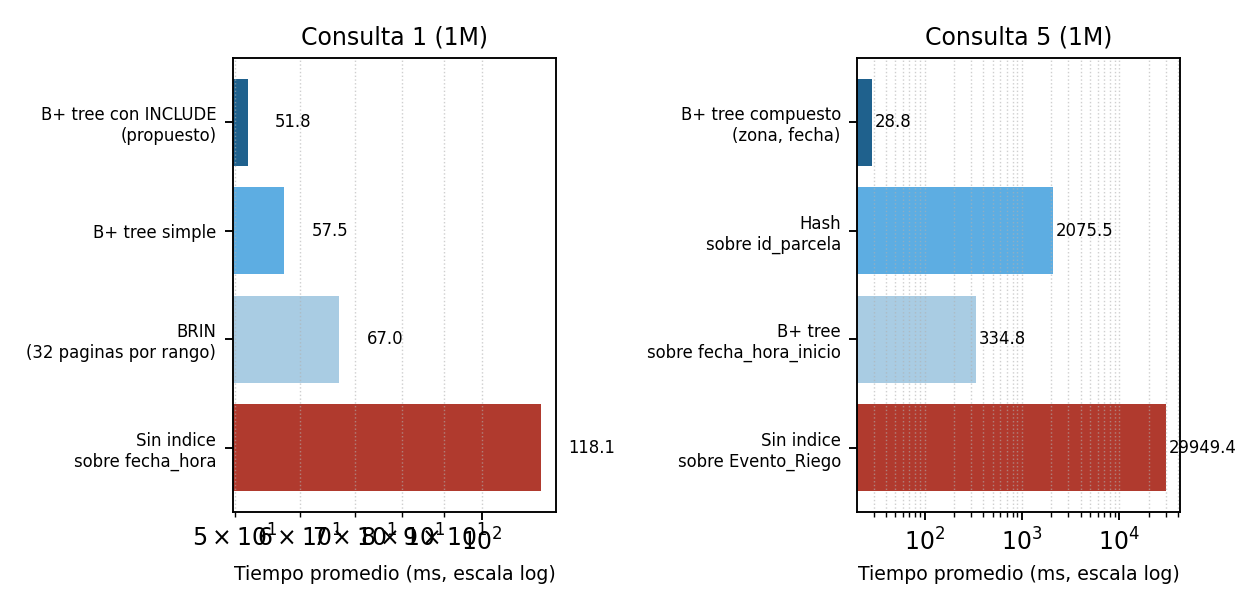
\includegraphics[width=0.95\textwidth]{figuras/tipos_indice.png}
\caption{Tiempo promedio según el tipo de índice (1M, escala logarítmica).}
\end{figure}

El resultado más útil para este dominio es el del BRIN. Guarda solo el valor mínimo y máximo de la fecha por cada bloque de 32 páginas, por eso ocupa 24~KB frente a los casi 30~MB del B+ tree con \tb{INCLUDE}, y se construye cinco veces más rápido. Aun así logra el 77~\% de la mejora del B+ tree (67~ms frente a 52~ms, partiendo de 118~ms). Funciona porque las lecturas están guardadas en orden cronológico: cada bloque contiene un intervalo de tiempo estrecho y el índice descarta la mayoría de bloques sin leerlos. Si las lecturas llegaran desordenadas, el BRIN no serviría.

En la consulta 5, el hash sobre la parcela solo resuelve la primera igualdad: encuentra todos los riegos de la parcela y debe filtrar zona y fecha fila por fila, por eso tarda 72 veces más que el B+ tree compuesto. El B+ tree sobre la fecha recorre el rango de seis horas de toda la empresa y filtra la zona, lo que lo deja en un punto intermedio. Un índice solo es tan bueno como su coincidencia con el patrón de búsqueda: el orden y la combinación de columnas pesan más que el tipo de estructura.

\subsubsection{Costo de los índices en las operaciones de escritura}

%%TABLA_ESCRITURA%%

\begin{figure}[H]
\centering
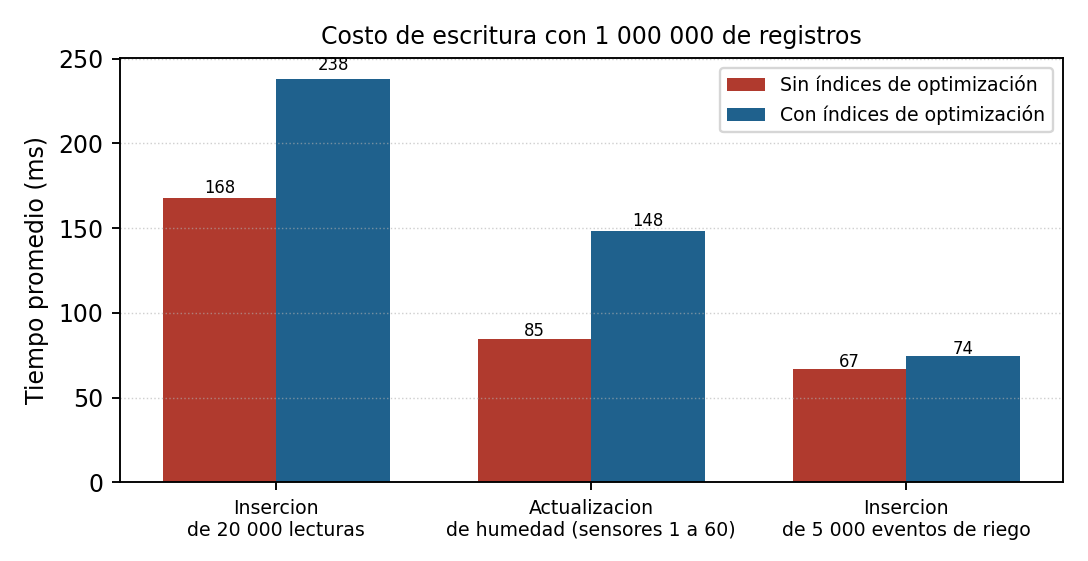
\includegraphics[width=0.78\textwidth]{figuras/escritura.png}
\caption{Tiempo de las operaciones de escritura con y sin índices de optimización (1M).}
\end{figure}

Los índices tienen un precio. Insertar 20\,000 lecturas cuesta 42~\% más con los índices de optimización, porque cada fila debe insertarse en tres árboles en lugar de uno. La actualización de humedad es la más afectada (75~\%): la columna \tb{humedad\_pct} está incluida en dos índices, así que PostgreSQL no puede hacer una actualización HOT (en la misma página, sin tocar índices) y debe escribir una entrada nueva en cada índice. En \tb{Evento\_Riego}, con un solo índice adicional, el sobrecosto es de 12~\%. La Tabla~\ref{tab:tamidx} muestra el espacio que ocupa cada índice.

%%TABLA_INDICES_TAM%%

\subsection{Resultados}

\subsubsection{Consulta 1}

\begin{figure}[H]
\centering
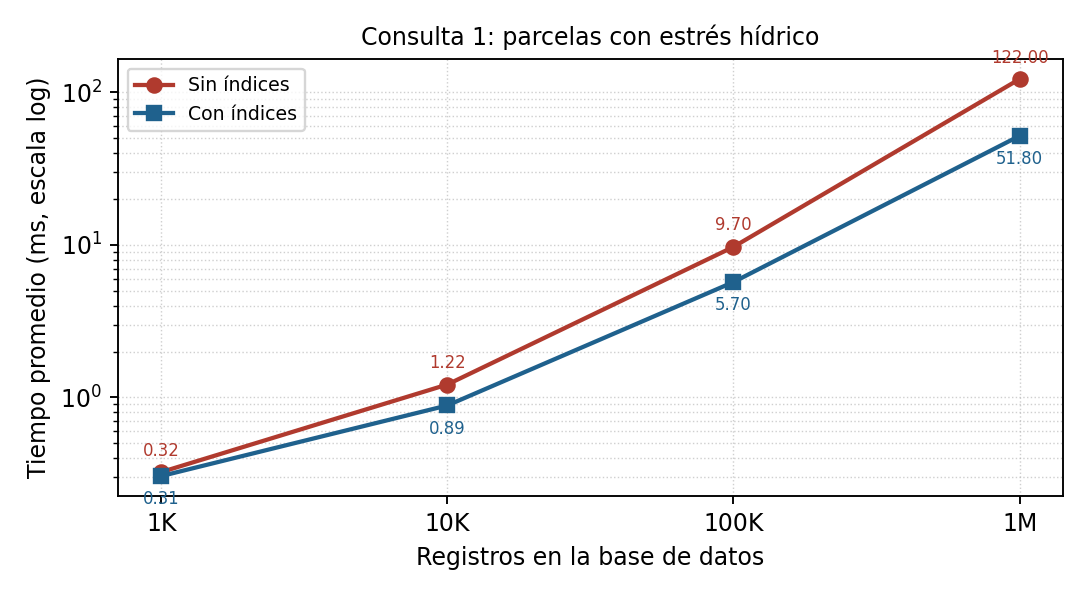
\includegraphics[width=0.78\textwidth]{figuras/consulta1.png}
\caption{Consulta 1: tiempo promedio por escenario.}
\end{figure}

%%RESUMEN_Q:1%%

El índice mejora la consulta a partir de 10\,000 registros y con un millón la acelera 2.4 veces. Sin índice, PostgreSQL recorre las 765\,861 lecturas con un \emph{Parallel Seq Scan} y descarta nueve de cada diez. Con el índice, el \emph{Index Only Scan} sobre \tb{idx\_lectura\_fecha} lee solo las 77\,020 lecturas del último mes. Los índices sobre campañas y dispositivos no se usan: esas tablas tienen pocos miles de filas y el planificador las recorre completas porque le resulta más barato.

\textbf{Plan de ejecución sin índices (1M)}
%%PLAN:1:sin%%
\textbf{Plan de ejecución con índices (1M)}
%%PLAN:1:con%%

\subsubsection{Consulta 2}

\begin{figure}[H]
\centering
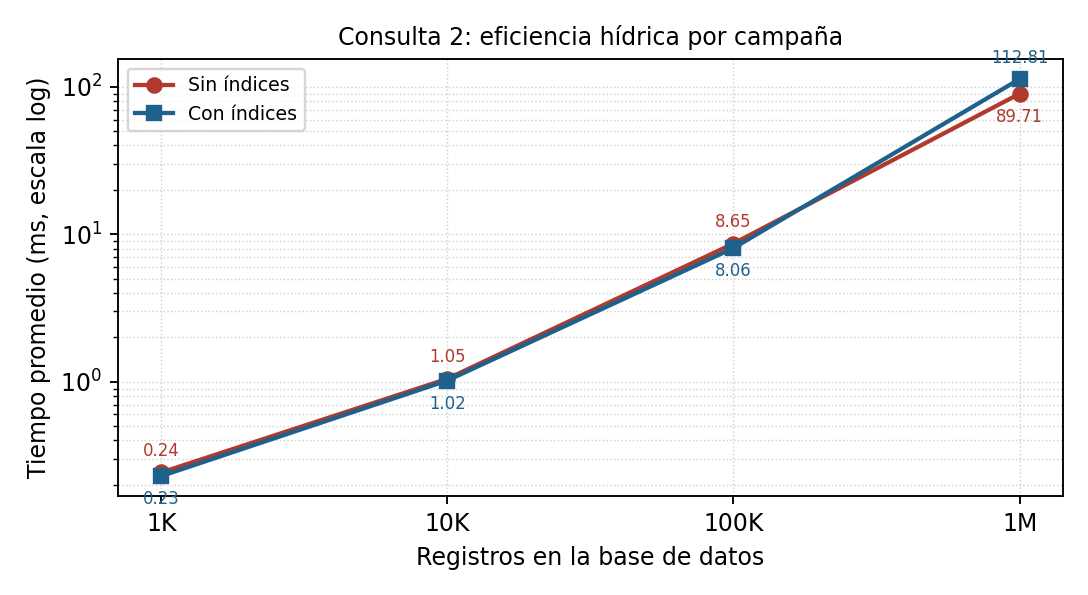
\includegraphics[width=0.78\textwidth]{figuras/consulta2.png}
\caption{Consulta 2: tiempo promedio por escenario.}
\end{figure}

%%RESUMEN_Q:2%%

Es el caso en que el índice perjudica. Hasta 100\,000 registros la versión con índices es ligeramente más rápida, pero con un millón es 26~\% más lenta. Sin índices, el plan lee una sola vez los 120\,000 riegos y los une con las campañas mediante un \emph{Hash Join}. Con índices, el planificador cambia a un \emph{Nested Loop}: por cada una de las 1\,500 campañas desciende por \tb{idx\_evento\_parcela\_fecha} y agrega un nodo \emph{Memoize} para reutilizar búsquedas repetidas. Ese caché no acierta ni una vez (0 aciertos, 1\,500 fallos) porque cada campaña tiene un rango de fechas distinto. Mil quinientos descensos por el índice más el costo del caché inútil superan a un único recorrido secuencial. El planificador estimó mal y solo la medición lo revela.

\textbf{Plan de ejecución sin índices (1M)}
%%PLAN:2:sin%%
\textbf{Plan de ejecución con índices (1M)}
%%PLAN:2:con%%

\subsubsection{Consulta 3}

\begin{figure}[H]
\centering
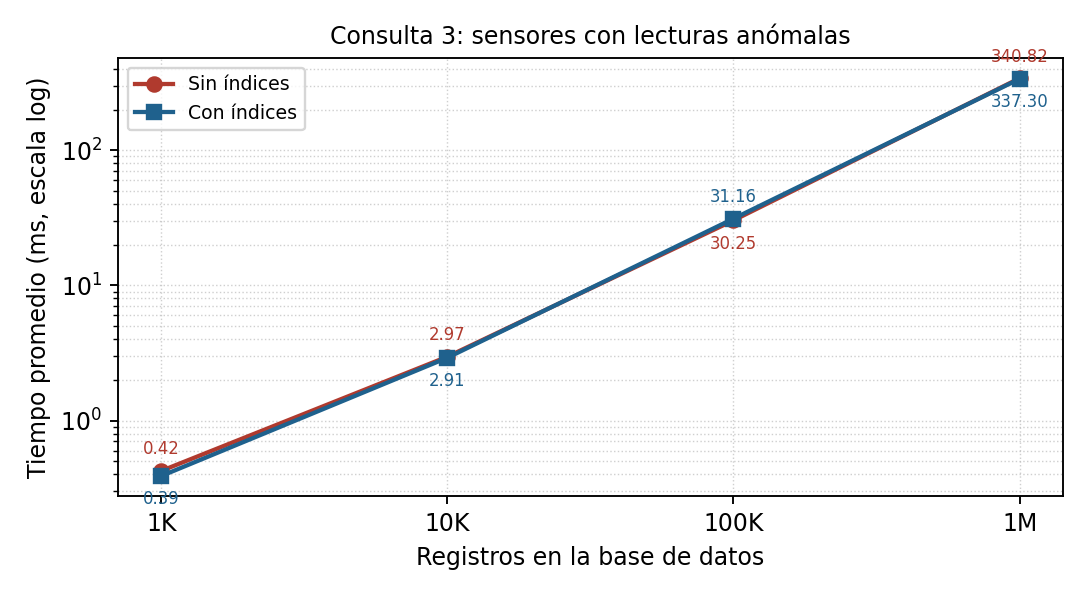
\includegraphics[width=0.78\textwidth]{figuras/consulta3.png}
\caption{Consulta 3: tiempo promedio por escenario.}
\end{figure}

%%RESUMEN_Q:3%%

Los tiempos son prácticamente iguales en las dos condiciones y el plan es el mismo: un recorrido secuencial paralelo de toda la tabla de lecturas. La consulta necesita el 84~\% de las filas, y para ese volumen leer la tabla en orden físico es más barato que recorrer un índice. El índice \tb{idx\_lectura\_disp\_humedad} ocupa 24~MB y nunca se usa.

\textbf{Plan de ejecución sin índices (1M)}
%%PLAN:3:sin%%
\textbf{Plan de ejecución con índices (1M)}
%%PLAN:3:con%%

\subsubsection{Consulta 4}

\begin{figure}[H]
\centering
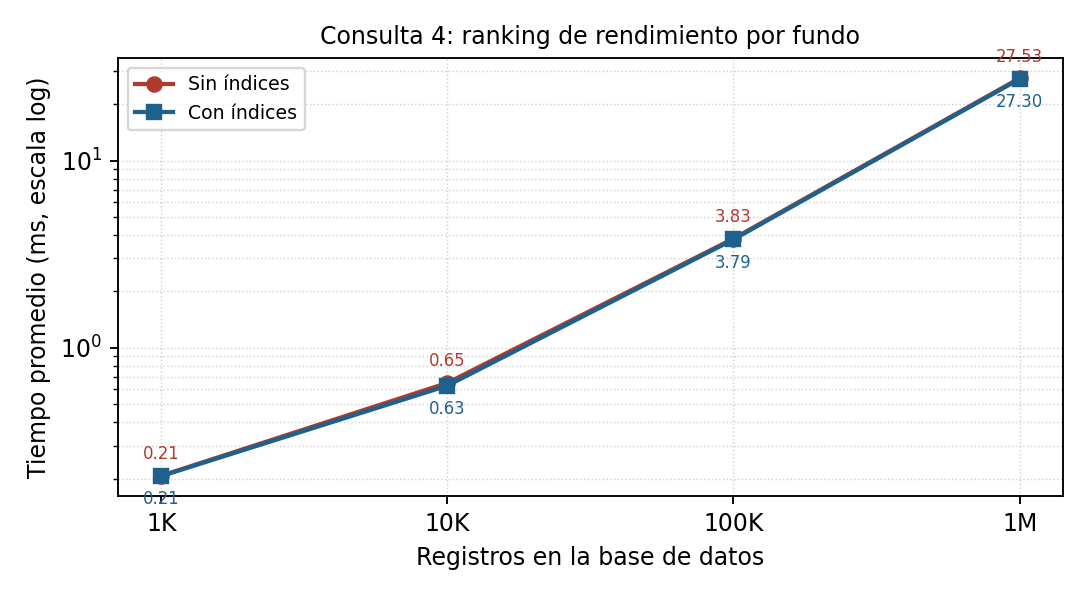
\includegraphics[width=0.78\textwidth]{figuras/consulta4.png}
\caption{Consulta 4: tiempo promedio por escenario.}
\end{figure}

%%RESUMEN_Q:4%%

Tampoco hay diferencia. El filtro por categoría conserva el 82~\% de las cosechas (primera y segunda), así que el planificador vuelve a preferir el recorrido secuencial, y la tabla de cosechas es pequeña (25\,000 filas). La mayor parte del tiempo se va en las funciones de ventana y en el ordenamiento, que ningún índice acelera en este caso.

\textbf{Plan de ejecución sin índices (1M)}
%%PLAN:4:sin%%
\textbf{Plan de ejecución con índices (1M)}
%%PLAN:4:con%%

\subsubsection{Consulta 5}

\begin{figure}[H]
\centering
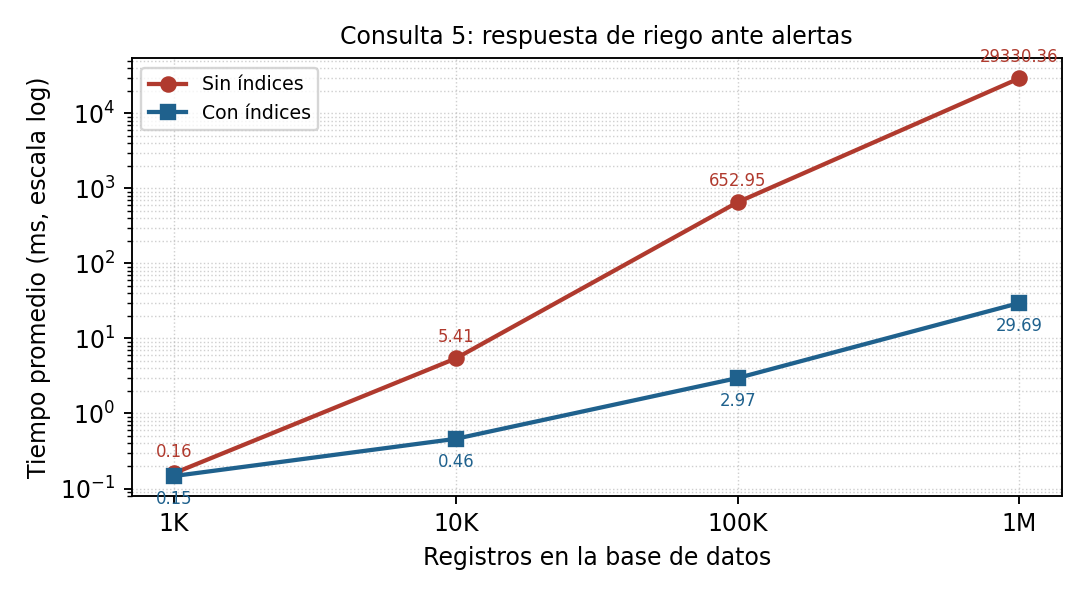
\includegraphics[width=0.78\textwidth]{figuras/consulta5.png}
\caption{Consulta 5: tiempo promedio por escenario.}
\end{figure}

%%RESUMEN_Q:5%%

Es la mejora más grande del experimento: con un millón de registros la consulta pasa de 29 segundos a 30 milisegundos, casi mil veces más rápida. Sin índice, la subconsulta correlacionada ejecuta un recorrido secuencial de \tb{Evento\_Riego} por cada una de las 7\,714 alertas y descarta en promedio unas 60\,000 filas en cada uno. Con índice, cada búsqueda es un \emph{Index Only Scan} sobre \tb{uq\_evento} que tarda alrededor de un microsegundo. La brecha crece con el volumen: 12 veces en 10\,000 registros, 220 veces en 100\,000 y casi mil en un millón.

\textbf{Plan de ejecución sin índices (1M)}
%%PLAN:5:sin%%
\textbf{Plan de ejecución con índices (1M)}
%%PLAN:5:con%%

\subsection{Análisis y Discusión}
\label{sec:discusion}

\begin{figure}[H]
\centering
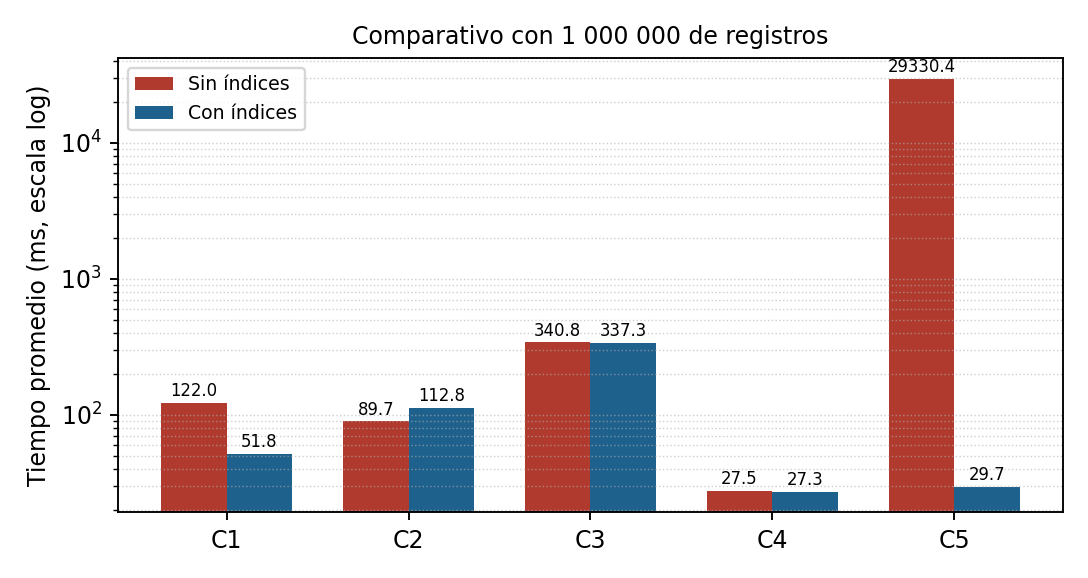
\includegraphics[width=0.78\textwidth]{figuras/comparativo1m.png}
\caption{Comparación de las cinco consultas con un millón de registros.}
\end{figure}

%%TABLA_RESUMEN%%

\textbf{Los índices no mejoran todo.} De las cinco consultas, dos mejoran de forma clara, dos no cambian y una empeora. De los nueve índices propuestos, el planificador solo eligió tres en el escenario de un millón (\tb{idx\_lectura\_fecha}, \tb{idx\_alerta\_humedad\_baja} e \tb{idx\_evento\_parcela\_fecha}), y el tercero hizo más lenta la consulta 2. Los otros seis ocupan espacio y encarecen las escrituras sin aportar nada a estas consultas. La Tabla~\ref{tab:planes} resume qué método de acceso usó el plan en cada escenario.

%%TABLA_PLANES%%

\textbf{Cuándo ayuda un índice.} Ayuda cuando la consulta necesita una fracción pequeña de una tabla grande (consulta 1, el último mes) o cuando debe repetir muchas búsquedas puntuales (consulta 5, una por alerta). No ayuda cuando la consulta lee casi toda la tabla (consultas 3 y 4) ni cuando la tabla es tan pequeña que cabe en pocas páginas, como \tb{Campania} con 1\,500 filas. En los escenarios de mil y diez mil registros casi no hay diferencias por la misma razón: todo cabe en memoria y cualquier plan termina en fracciones de milisegundo.

\textbf{El planificador puede equivocarse.} La consulta 2 muestra que un índice razonable puede empeorar el tiempo. El planificador elige con estimaciones de costo, y cuando la estimación falla, como con el \emph{Memoize} sin aciertos, el plan resultante es peor. Además, el efecto se invirtió entre escenarios: con 100\,000 registros el índice ayudaba un poco. Cada índice debe validarse con \tb{EXPLAIN ANALYZE} en un volumen representativo, no darse por bueno en teoría.

\textbf{Optimización lógica y física.} La consulta 5 repite la misma subconsulta \tb{EXISTS} en dos lugares, así que se evalúa dos veces por alerta. La reescribimos para evaluarla una sola vez dentro de una CTE (Tabla~\ref{tab:reescritura}).

%%TABLA_REESCRITURA%%

La primera reescritura no mejoró nada, y la causa es una característica de PostgreSQL que conviene conocer: desde la versión 12, una CTE que se usa una sola vez se incrusta en la consulta principal, y al hacerlo la expresión \tb{EXISTS} volvió a aparecer en los dos agregados. El plan lo confirma: siguen existiendo dos subconsultas y no aparece ningún \emph{CTE Scan}. Al declarar la CTE como \tb{MATERIALIZED}, la subconsulta se evalúa una sola vez y el tiempo sin índices baja a la mitad. Es una mejora real, pero pequeña frente al índice: reescribir divide el tiempo entre dos y el índice lo divide entre mil. Lo ideal es combinar ambas cosas.

%%SQL_ARCHIVO:03c_consulta5_materializada.sql%%

\textbf{Resumen práctico.} Para esta base recomendamos conservar \tb{idx\_lectura\_fecha} (o su versión BRIN si el espacio importa) e \tb{idx\_alerta\_humedad\_baja}, y retirar los otros siete. En particular, \tb{idx\_lectura\_disp\_humedad} ocupa 24~MB, nunca se usa y encarece cada actualización de humedad.

\subsection{Complejidad operacional por encima del millón de registros}
\label{sec:extra}

\textbf{Cómo crece cada consulta.} La Tabla~\ref{tab:crecimiento} muestra cuántas veces aumenta el tiempo cuando los datos se multiplican por diez. Si el factor es cercano a 10, el crecimiento es lineal; si se acerca a 100, es cuadrático. El exponente $b$ resume el último tramo: el tiempo crece como $n^b$.

%%TABLA_CRECIMIENTO%%

Casi todas las consultas crecen de forma lineal ($b \approx 1$), lo que corresponde a recorridos completos de tabla con uniones hash: el costo es proporcional al número de filas. La excepción es la consulta 5 sin índice, con exponentes entre 1.6 y 2.1. La razón es que el número de alertas y el de riegos crecen a la vez, y por cada alerta se recorre la tabla de riegos: el costo es $O(A \cdot E)$, que en la práctica es cuadrático. Con el índice, cada búsqueda cuesta $O(\log E)$ y el total queda en $O(A \log E)$, casi lineal, como confirma el exponente de 1.0.

\textbf{Proyección.} Si extrapolamos esos exponentes, con diez millones de registros la consulta 5 sin índice pasaría de 30 segundos a entre 20 y 60 minutos, mientras que con índice rondaría los 300~ms. La consulta 1 sin índice subiría a alrededor de un segundo y medio. Son estimaciones gruesas, porque al crecer la base dejaría de caber en memoria y aparecerían lecturas de disco que hoy no existen, pero el orden de magnitud basta para ver que los recorridos completos dejan de ser una opción.

\textbf{Volumen real esperado.} Con los @@SENSORES@@ sensores reportando cada 15 minutos, la tabla de lecturas recibiría unos @@LECTANIO@@ millones de filas al año (alrededor de @@GBANIO@@ GB con los índices actuales). El ritmo de escritura no es el problema: equivale a unas 2.4 lecturas por segundo, y en la prueba de escritura insertamos 20\,000 lecturas en 238~ms, unas 84\,000 por segundo con todos los índices. Aunque registrar fila por fila con el trigger de alertas es mucho más lento que una inserción masiva, el margen es de varios órdenes de magnitud. El problema está en las consultas analíticas sobre años de historia. Incluso la consulta 1 con índice escala con el tamaño de la ventana consultada: con la frecuencia real, un mes tendría unos 6.3 millones de lecturas, y leerlas por índice tomaría varios segundos.

\textbf{¿Es suficiente la arquitectura cliente-servidor?} Para el volumen de esta empresa, sí, siempre que el servidor se organice para ese crecimiento. En orden de prioridad:

\begin{enumerate}[leftmargin=1.6em,itemsep=0.15em]
\item \textbf{Particionamiento por rango de fecha.} Dividir \tb{Lectura\_Suelo} en particiones mensuales con el particionamiento declarativo de PostgreSQL. Una consulta del último mes solo toca una partición (\emph{partition pruning}), y las particiones antiguas pueden archivarse o desconectarse sin borrar fila por fila.
\item \textbf{BRIN por partición.} Como los datos llegan en orden cronológico, un BRIN sobre la fecha cuesta kilobytes en lugar de megabytes y casi iguala al B+ tree, como medimos.
\item \textbf{Agregados materializados.} Una vista materializada con el resumen diario por sensor (promedio, mínimo, máximo y conteo), refrescada cada noche. Las consultas 1 y 3 leerían unas 2\,200 filas por día en lugar de 211\,000 lecturas.
\item \textbf{Réplica de lectura.} Una réplica por \emph{streaming replication} para los reportes de gerencia, de modo que las consultas pesadas no compitan con la ingesta.
\item \textbf{Extensiones especializadas.} Si el volumen creciera mucho más, TimescaleDB añade a PostgreSQL particionamiento automático, compresión y agregados continuos para series de tiempo, sin salir del modelo relacional.
\end{enumerate}

El modelo cliente-servidor dejaría de ser suficiente en otro escenario: una plataforma que atienda a miles de fundos de distintas empresas, con miles de millones de filas por año, alta disponibilidad entre regiones o análisis que recorran terabytes. Ahí el lado del servidor tendría que convertirse en un clúster distribuido o apoyarse en un almacén columnar para la analítica. Aun así, los clientes seguirían hablando con un servicio; lo que cambia es que ese servicio ya no es una sola máquina.

% ================================================================== 6
\section{Conclusiones}

\begin{enumerate}[leftmargin=1.6em,itemsep=0.25em]
\item El modelo cubre el dominio con una especialización total y disjunta, dos entidades débiles y una relación ternaria. El esquema resultante está en tercera forma normal. La única tabla que no cumple FNBC (\tb{Evento\_Riego}) se dejó así a propósito para preservar dependencias, y la dependencia se controla con un trigger.
\item Llevar las reglas del negocio a la base de datos funcionó. Restricciones, procedimientos y triggers rechazaron todas las operaciones inválidas de las pruebas, y las verificaciones de consistencia encontraron errores del generador que habrían contaminado el experimento.
\item Los índices no son una mejora universal. Solo dos de las cinco consultas se aceleraron (2.4 y casi mil veces), dos no cambiaron y una se volvió 26~\% más lenta. Solo tres de los nueve índices propuestos llegaron a usarse.
\item La mayor ganancia aparece en las subconsultas correlacionadas: el índice convierte un costo cuadrático en uno casi lineal, y la diferencia crece con el volumen.
\item Para series de tiempo guardadas en orden de llegada, un BRIN ofrece casi el mismo beneficio que un B+ tree con una fracción mínima del espacio. En un sistema IoT que crece de forma indefinida, esa diferencia pesa.
\item Todo índice cuesta en escritura, entre 12 y 75~\% en nuestras pruebas, y el peor caso aparece al actualizar columnas incluidas en índices. En tablas que reciben datos de forma continua, cada índice debe justificarse con mediciones.
\item La optimización lógica también cuenta, pero hay que verificarla. Reescribir la consulta 5 no sirvió hasta forzar la materialización de la CTE; después, redujo el tiempo a la mitad.
\item La arquitectura cliente-servidor basta para el volumen previsto si se combina con particionamiento por fecha, índices BRIN y agregados materializados. Las alternativas distribuidas solo se justificarían con una escala varios órdenes de magnitud mayor.
\end{enumerate}

% ================================================================== 7
\section{Anexos}

\subsection{Video de demostración}

Video con la base de un millón de registros, ejecutando las consultas con y sin índices: \enlaceVideo

Los comandos que se muestran en el video son los siguientes:

\begin{lstlisting}
-- 1. Restaurar el respaldo (desde la terminal)
--    createdb agro1m
--    pg_restore -d agro1m agro_1M.dump
-- 2. Comprobar el volumen
SELECT (SELECT count(*) FROM Lectura_Suelo) AS lecturas,
       (SELECT count(*) FROM Evento_Riego)  AS riegos,
       (SELECT count(*) FROM Alerta)        AS alertas;
-- 3. Consulta 5 sin indices
SET enable_indexscan = OFF; SET enable_bitmapscan = OFF; SET enable_indexonlyscan = OFF;
EXPLAIN ANALYZE <consulta 5>;
-- 4. Consulta 5 con indices
SET enable_indexscan = ON; SET enable_bitmapscan = ON; SET enable_indexonlyscan = ON;
EXPLAIN ANALYZE <consulta 5>;
\end{lstlisting}

\subsection{Respaldos de la base de datos}

Los cuatro respaldos se generaron con \tb{pg\_dump} en formato personalizado y compresión nivel 6: \enlaceDumps

%%TABLA_DUMPS%%

Para restaurar uno de ellos: \tb{createdb agro1m} y luego \tb{pg\_restore -d agro1m agro\_1M.dump}.

\subsection{Scripts del proyecto}

Carpeta con todos los scripts: \enlaceRepositorio

\begin{table}[H]
\centering\small
\begin{tabularx}{\textwidth}{>{\raggedright\arraybackslash}p{5.4cm}X}
\toprule
\textbf{Archivo} & \textbf{Contenido} \\
\midrule
\tb{sql/01\_ddl.sql} & Creación de las 18 tablas con sus restricciones. \\
\tb{sql/01b\_comentarios.sql} & Documentación de tablas y columnas (fuente del diccionario). \\
\tb{sql/02\_vistas\_procedimientos\_triggers.sql} & Vistas, procedimientos, funciones y triggers. \\
\tb{sql/03\_consultas.sql} & Las cinco consultas del experimento. \\
\tb{sql/03b\_consulta5\_reescrita.sql}, \tb{03c\ldots} & Reescrituras de la consulta 5. \\
\tb{sql/04\_indices.sql} & Los nueve índices de optimización. \\
\tb{sql/05\_roles.sql} & Roles y permisos (opcional). \\
\tb{sql/06\_pruebas.sql} & Pruebas de procedimientos y triggers. \\
\tb{sql/07\_verificacion.sql} & Verificación de consistencia posterior a la carga. \\
\tb{scripts/generar\_datos.py} & Generador de datos sintéticos. \\
\tb{scripts/ejecutar\_todo.py} & Orquestador: carga, experimento y gráficos. \\
\tb{scripts/experimento.py} & Mediciones, reanudables por tramos. \\
\tb{scripts/graficos.py} & Figuras del informe. \\
\tb{scripts/construir\_informe.py} & Genera las tablas y listados de este informe desde los resultados. \\
\bottomrule
\end{tabularx}
\caption{Archivos entregados.}
\end{table}

\subsection{Generador de datos}
\label{sec:generador}

%%CODIGO_GENERADOR%%

\end{document}
